\documentclass{article}
\usepackage{amsmath,epsfig,calc,capt-of,ifthen}
\usepackage{psfig, amsmath, amsthm, amssymb, epsfig}
\usepackage{graphicx}


%%%%%%%%%% Start TeXmacs macros
\newcommand{\tmop}[1]{\ensuremath{\operatorname{#1}}}
\newcommand{\tmfloatcontents}{}
\newlength{\tmfloatwidth}
\newcommand{\tmfloat}[5]{
  \renewcommand{\tmfloatcontents}{#4}
  \setlength{\tmfloatwidth}{\widthof{\tmfloatcontents}+1in}
  \ifthenelse{\equal{#2}{small}}
    {\ifthenelse{\lengthtest{\tmfloatwidth > \linewidth}}
      {\setlength{\tmfloatwidth}{\linewidth}}{}}
    {\setlength{\tmfloatwidth}{\linewidth}}
  \begin{minipage}[#1]{\tmfloatwidth}
    \begin{center}
      \tmfloatcontents
      \captionof{#3}{#5}
    \end{center}
  \end{minipage}}
%%%%%%%%%% End TeXmacs macros

\begin{document}



\title{\bf \Large The Relationship Between the Recontructed Volume Coordinate System (RVCS),
Bio-Tree Standard Coordinate System (BSCS) and the Grid Coordinate System (GCS)}
\author{Kongbin Kang and H. Can Aras}\maketitle

\noindent The images reconstructed by filtered backprojection give us a coarse level
description of 3D geometric structure. It is useful using the
recontructed image to help an end-user to specify the region of interest for
our forward projection. This process requires a good understanding of the
relationship between RVCS and BSCS.

\section{The Reconstructed Volume Coordinate System}

\noindent As shown in Fig(\ref{fig:cali-rics}), the volume reconstructed by filtered backprojection
define a coordinate system - the origin is
located at the corner of the 3D volume. The $x$ and $y$ axis are parallel to a
recontructed image row and column, respectively. Then, the $z$ axis is defined by the
right-hand rule.\\

\tmfloat{h}{small}{figure}{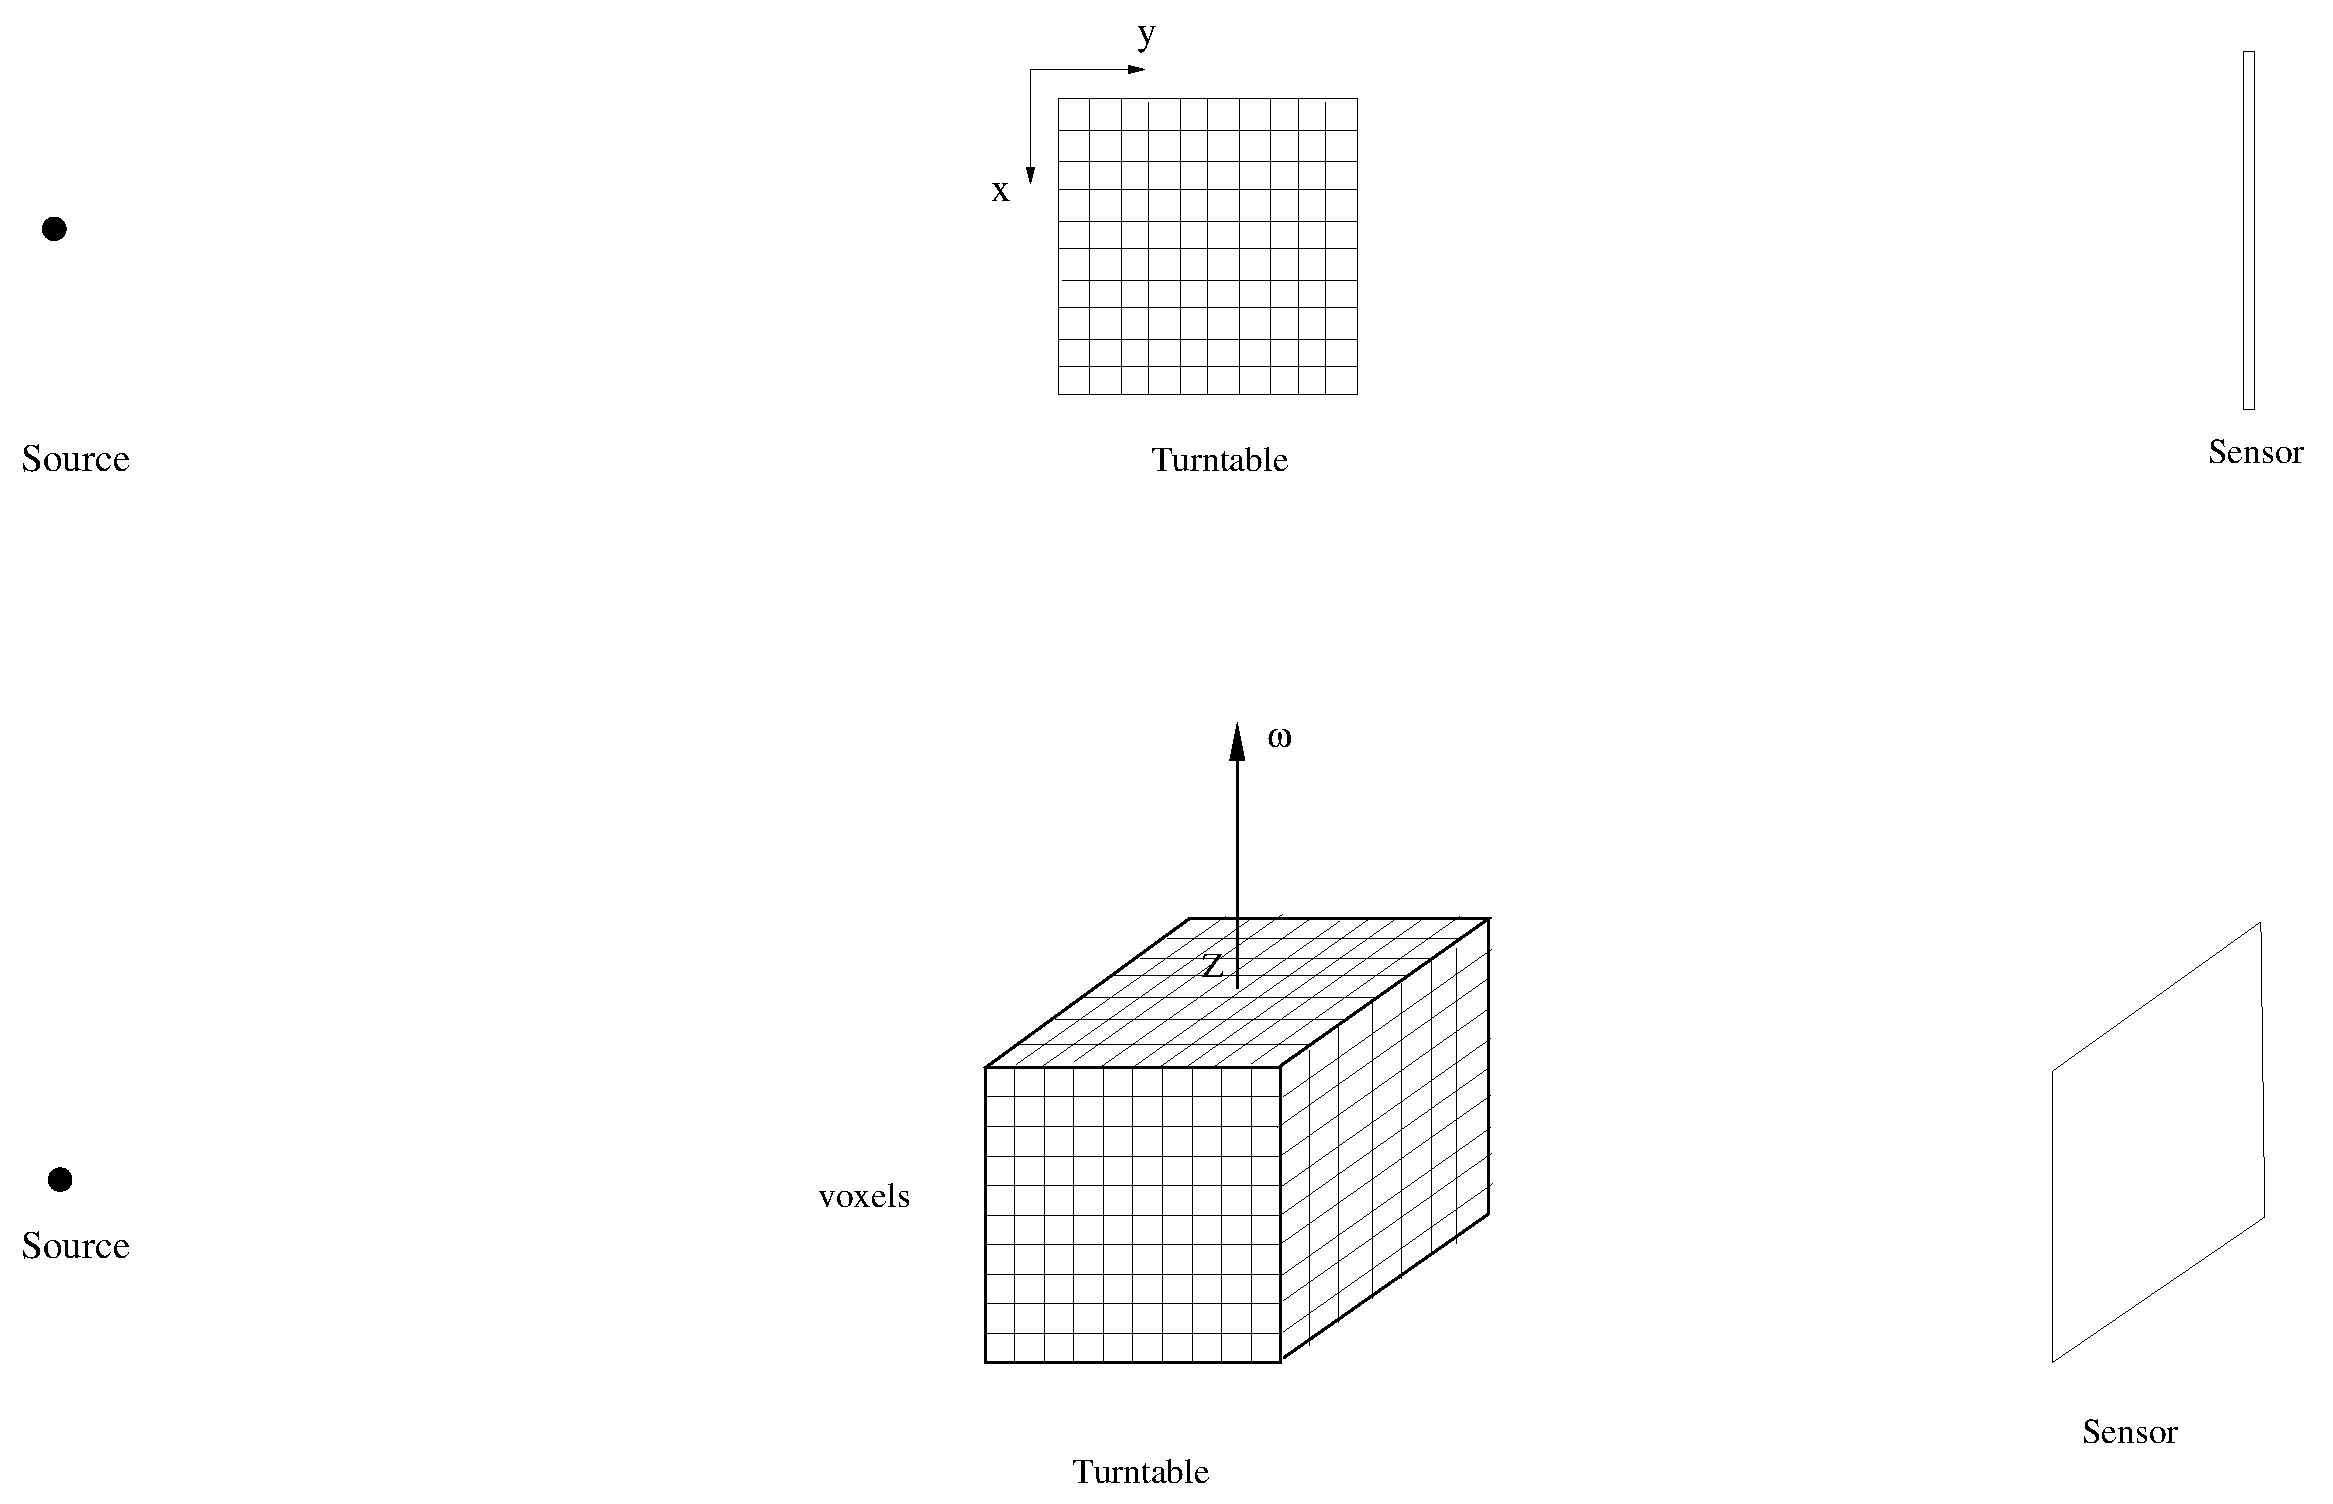
\epsfig{file=cali-1.eps, height=6.0cm}
}{\label{fig:cali-rics}A scan setup together with the top view.}

\section{Bio-Tree Standard Coordinate System}

\noindent See BioTreeStandartCoordinates.ppt file by Prof. Joseph Mundy for
an explanation on this topic.

\section{The Aligment Between the Two Coordinate Systems}

\noindent The aligment is given as follows:
\begin{equation*}
  \left(\begin{array}{c}
    x_b\\
    y_b\\
    z_b
  \end{array}\right) = \left(\begin{array}{c}
    \alpha_{} (x - \frac{n_x}{2})\\
    \alpha_{} (y - \frac{n_y}{2})\\
    \frac{a}{b} \beta_v (z - (s_v - v_0))
  \end{array}\right),
\end{equation*}
where $x_b$, $y_b$ and $z_b$ represent the coordinates in Bio-Tree coordinate
system; $x$, $y$ and $z$ represent the coordinates in the reconstructed coordinate
system; $\alpha$ is the reconstructed voxel size; $a$ and $b$ are the rotation center to source
and sensor to source distances respectively; $s_v$ is the projected view dimension along
vertical direction. $\beta_v$ is sensor pixel size along the vertical direction, $v_0$ is the
principle point on the sensor along the vertical direction; $(n_x, n_y)$ is the dimension of a
reconstructed slice along $x$ and $y$ directions, respectively.

\subsection{Sanity Check}

We have the following information in hand for a feature point:
\begin{center}
  \begin{table}[h]
    \begin{tabular}{|c|c|c|}
\hline
      Feature Point & Hair Crossing Center & Rotation Center\\
      \hline
      splating reconstruction result in BSCS (mm) & (-1.2792*2, 1.0479*2, x)
      & (0.0, 0.0, 0.0)\\
      \hline
      FBP reconstruction result (voxels) & (855, 1119, 347) & (1000, 1000,
      1000)\\
      \hline
    \end{tabular}
    \caption{A hair crossing feature point is measured in both RVCS and BSCS}
  \end{table}
\end{center}
\noindent Given $n_x = n_y = 2000$ and $\alpha = 17.70$um, $\beta_u = 11.70$um
and using the measurements from the reconstructed image, we get $x_b = -2.5665$, $y_b =
2.1063$. Comparing this with the splatted-reconstruction result in Bio-Tree Standard Coordinate
System, we get the error for this feature point as:
\[ \left(\begin{array}{c}
     \Delta x_b\\
     \Delta y_b\\
     \Delta z_b
   \end{array}\right) = \left(\begin{array}{c}
     - 0.008\\
     0.01050\\
     0
   \end{array}\right). \]


\subsection{Using the FBP Reconstruction to Define a Region of Interest in BSCS}

Given that $\alpha = 17.56570$, $\beta_u = 11.70$, $v_0 =
623$, $a = 261.50$ and $b = 345.712$, we get the following:
\begin{center}
  \begin{table}[h]
    \begin{tabular}{|c|c|c|}
\hline
      Feature Point & Hair Crossing Center & Rotation Center\\
      \hline
      splating reconstruction result in BSCS (mm) & (-2.8983, 1.1593, 0.9646)
      & (0.0, 0.0, 0.0)\\
      \hline
      FBP reconstruction result in (voxel) & (835,1066, 534) & (1000, 1000,
      1000)\\
      \hline
    \end{tabular}
    \caption{A hair crossing feature point is measured in both RVCS and BSCS}
  \end{table}
\end{center}
\section{Conversion from the Bio-Tree Standard Coordinate System
to the Grid Coordinate System}

The grid coordinate system is defined on the region of interest which is 
the user-defined 3D box. The coordinates of the grid coincides with the coordinates
of BSCS. The origin is at $(x_{min},y_{min},z_{min})$ of the 3D box. Given the coordinates
of a point in BSCS, we can find the grid coordinates using the following formula:

\begin{equation*}
  \left(\begin{array}{c}
    x_g\\
    y_g\\
    z_g
  \end{array}\right) = \left(\begin{array}{c}
    (x_b-x_{min})/r\\
    (y_b-y_{min})/r\\
    (z_b-z_{min})/r
  \end{array}\right),
\end{equation*}

\noindent where $x_b$, $y_b$ and $z_b$ represent the coordinates in Bio-Tree coordinate
system; $x_g$, $y_g$ and $z_g$ represent the grid coordinates; and $r$ is the resolution
used for our splatted-reconstruction.

\section{Conclusion}

From the above discussion, we can conclude that utilizing the filtered backprojection
result of SkyScan as a tool to define the region of interest is feasible, and 
the error of the alignment is within $10$um.

\end{document}

